\chapter{UML Project Diagrams}\label{ap:uml}


\begin{table}[ht!]
	\centering
	\caption{Components Implementation}
	\label{tab:components-implementation}
	\begin{tabular}{l r}
		\toprule
		\textbf{Component} & \textbf{Implementation}\\
		\midrule
		Sniffer			& Python \\
		Sqlite Database	& Python \\
		TraceAnalyzer	& C++ \\
		FlowGenerator	& C++ \\
		\bottomrule
	\end{tabular}
\end{table}




\begin{figure*}[h]
	\centering
	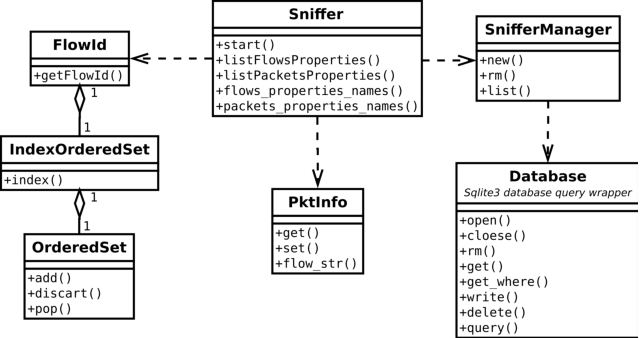
\includegraphics[width=0.8\textwidth]{figures/apD/sniffer}
	\caption{Sniffer UML Class Diagram}
	\label{fig:uml-sniffer}
\end{figure*}


\clearpage

\begin{figure*}[]
	\centering
	\begin{turn}{90}
	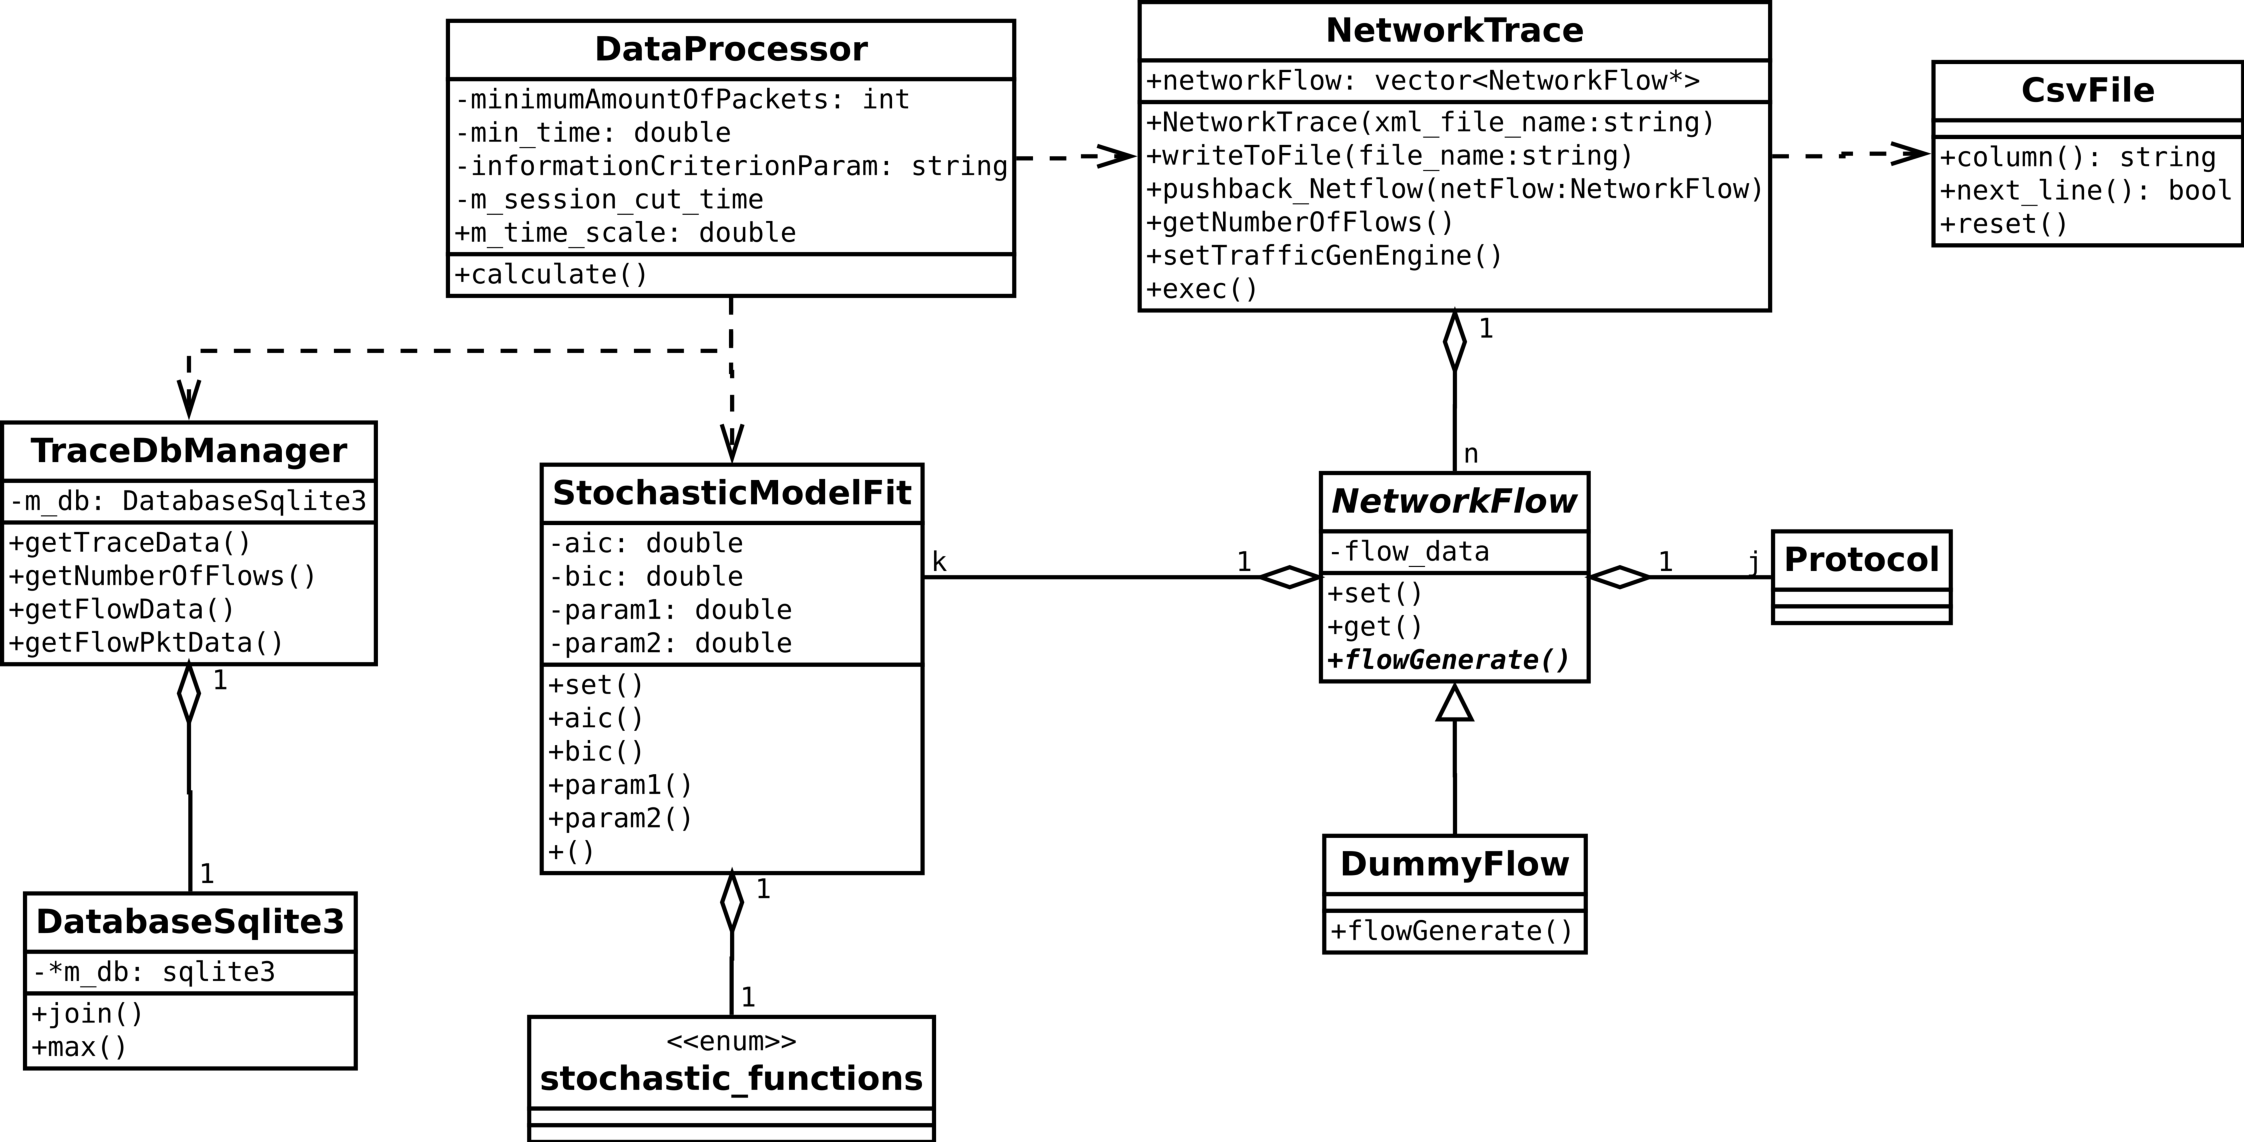
\includegraphics[width=1.5\textwidth]{figures/apD/trace-analyzer}
	\end{turn}
	\caption{TraceAnalyzer UML Class Diagram}
	\label{fig:uml-trace-analyzer}
\end{figure*}

\clearpage

\begin{figure*}[]
	\centering
	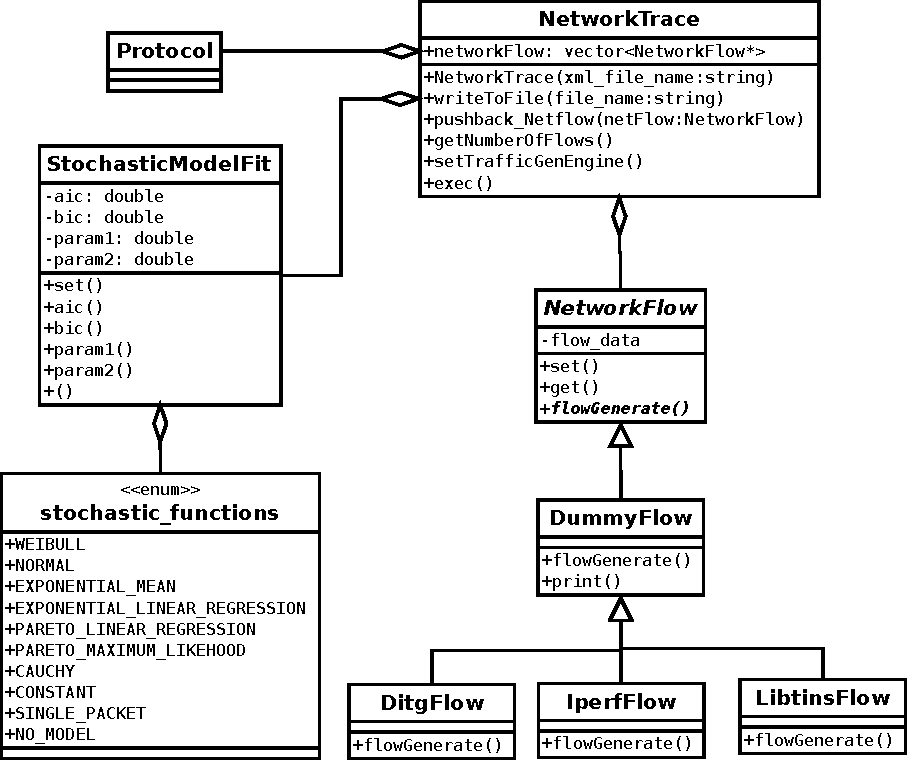
\includegraphics[width=0.9\textwidth]{figures/apD/flow-generator}
	\caption{FlowGenerator UML Class Diagram}
	\label{fig:uml-flow-generator}
\end{figure*}

